\setAuthor{Jaan Kalda}
\setRound{lõppvoor}
\setYear{2009}
\setNumber{G 5}
\setDifficulty{4}
\setTopic{Kinemaatika}

\prob{GPS}
Tervisesportlane kasutab GPS seadet oma jooksutreeningu tulemuste salvestamiseks.
Tema GPS seade määrab iga 15 sekundi järel jooksja täpse asukoha, mille põhjal arvutab ja salvestab GPS seade viimase 15 sekundi keskmise kiiruse
ning esitab saadud tulemused graafikul punktidena, mis on ühendatud sirglõikude abil.
Jooksja märkas lahti läinud ketsipaelu, peatus ja sidus paelad kinni. Tänu väikesele puhkusele jätkas ta jooksmist juba kiiremini, vt juuresolevat GPS-i esitatud graafikut. Kui kaua kestis peatus? Pidurdumiseks ning puhkusjärgselt kiirendamiseks kulunud
aeg lugeda tühiseks; jooksu kiirus oli konstantne nii enne peatust kui ka pärast seda.

\begin{center}
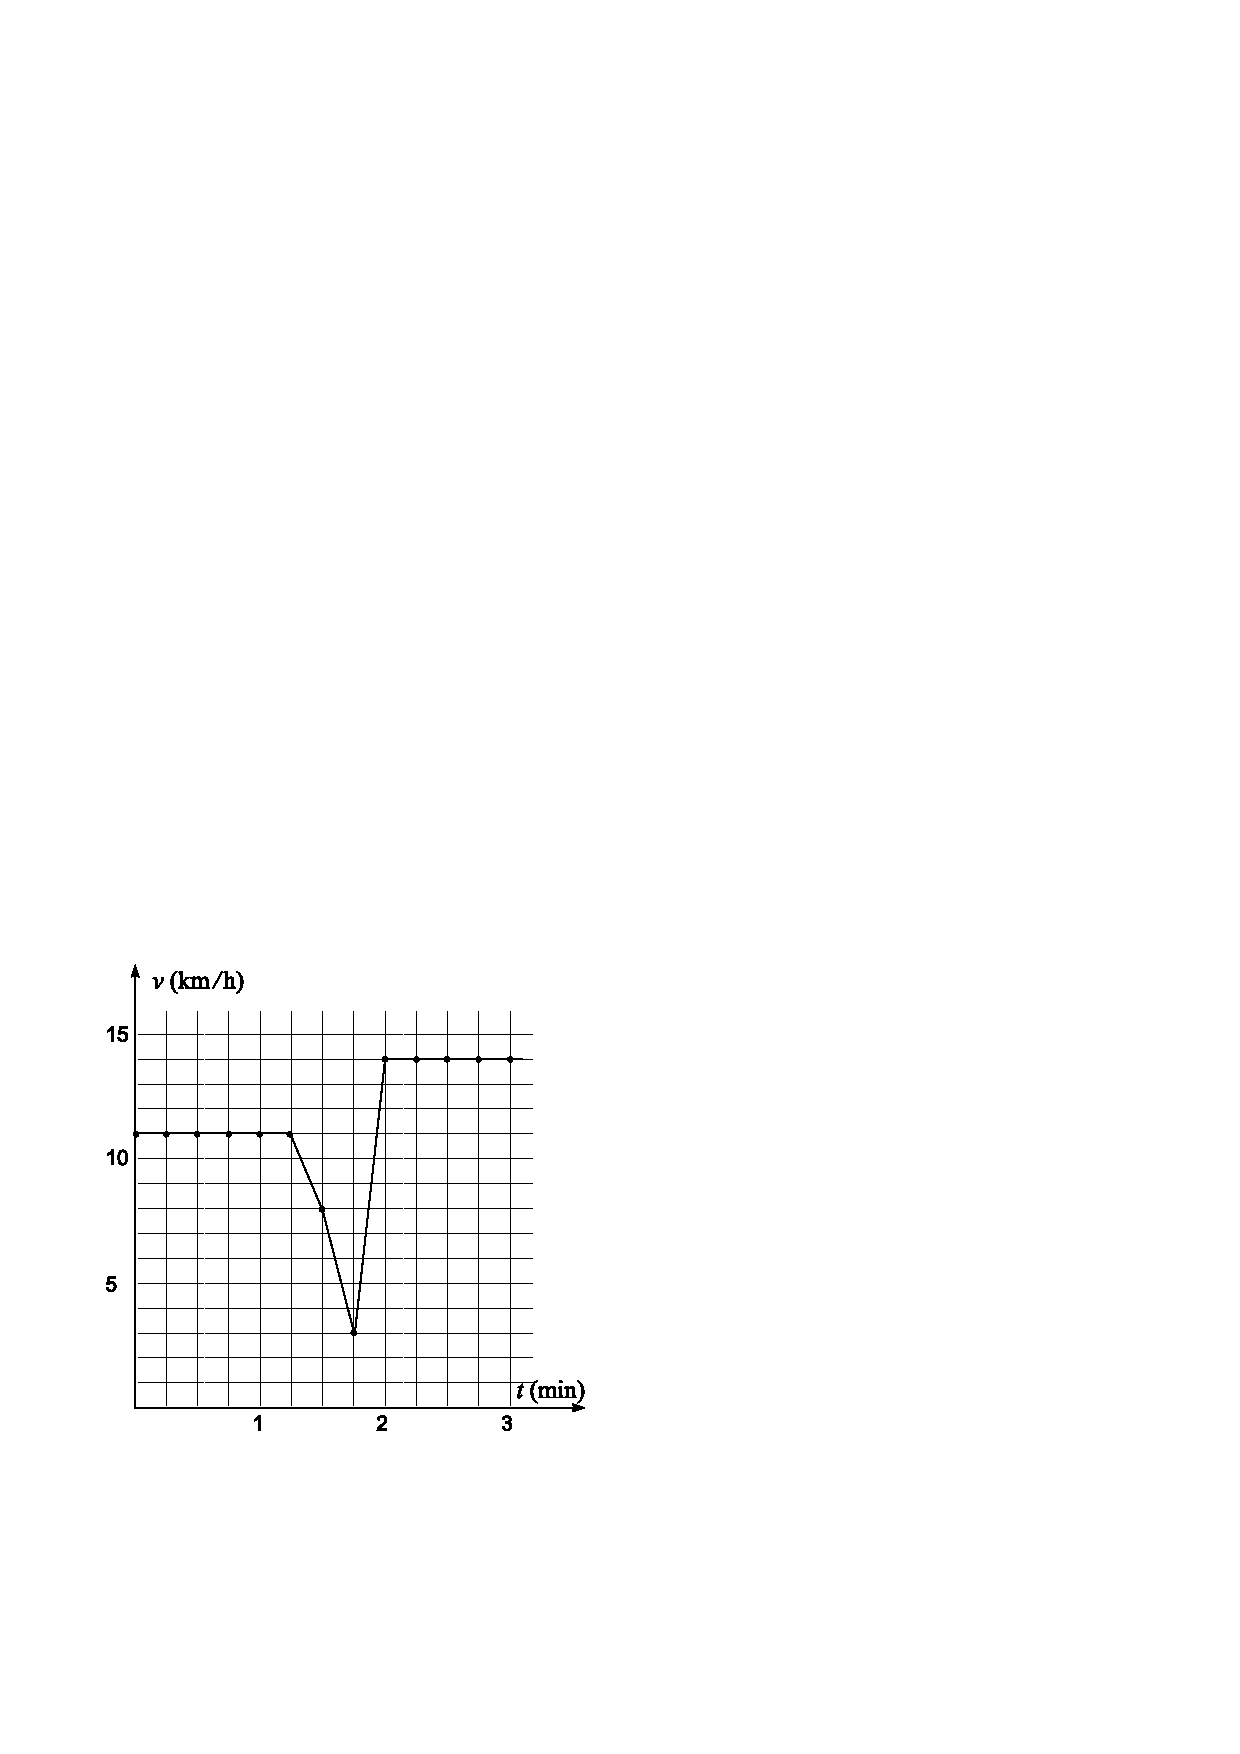
\includegraphics{2009-v3g-05-gps.pdf}
\end{center}\hint
Graafikult on näha, et ainult kahel mõõdetud ajahetkel oli sportlase kiirus keskmisest madalama väärtusega. See tähendab, et peatus mahtus täielikult antud kahe perioodi sisse.

\solu
Ajahetkel $t_1=\SI{75}s$ tervisesportlane veel jooksis, sest eelmise perioodi keskmine kiirus polnud veel alanenud ($v_0=\SI{11}{km/h}$);
et ajahetkeks $t_2=\SI {90}s$ oli keskmine kiirus langenud kiiruseni $v_1=\SI{8}{km/h}$, siis oli ta seisnud juba ajavahemiku
$\tau_1$, kus $v_1 T= v_0 (T-\tau_1)$ ning $T=\SI{15}{s}$. Seega, 
\[
\tau_1=\left(1-\frac{v_1}{v_0}\right)T.
\]
Analoogselt, pärast ajahetke $t_2$ seisis
sportlane veel ajavahemiku $\tau_2$, kus $v_2 T= v_3 (T-\tau_2)$ ning $v_2=\SI 3{km/h}$ ja $v_3=\SI{14}{km/h}$. Seega, 
\[
\tau_2=\left(1-\frac{v_2}{v_3}\right)T
\]
ning kogu peatusaeg
\[
\tau=\tau_1+\tau_2=T\left(2-\frac{v_1}{v_0}- \frac{v_2}{v_3}\right)\approx \SI{16}s.
\]
\probend